% Created 2020-08-03 Mon 00:24
% Intended LaTeX compiler: lualatex
\documentclass[11pt]{article}
\usepackage{graphicx}
\usepackage{grffile}
\usepackage{longtable}
\usepackage{wrapfig}
\usepackage{rotating}
\usepackage[normalem]{ulem}
\usepackage{amsmath}
\usepackage{textcomp}
\usepackage{amssymb}
\usepackage{capt-of}
\usepackage{hyperref}
\usepackage{tabularx}
\usepackage{etoolbox}
\makeatletter
\def\dontdofcolorbox{\renewcommand\fcolorbox[4][]{##4}}
\AtBeginEnvironment{minted}{\dontdofcolorbox}
\makeatother
\usepackage[newfloat]{minted}
\usepackage{pdfpages}
\author{Mark Armstrong}
\date{\today}
\title{Computer Science 3MI3 - Principles of Programming Languages\\\medskip
\large 2020 Course Outline}
\hypersetup{
   pdfauthor={Mark Armstrong},
   pdftitle={Computer Science 3MI3 - Principles of Programming Languages},
   pdfkeywords={},
   pdfsubject={The course outline for the 2020 class of 3mi3},
   pdfcreator={Emacs 27.0.90 (Org mode 9.3.7)},
   pdflang={English},
   colorlinks,
   linkcolor=blue,
   citecolor=blue,
   urlcolor=blue
   }
\begin{document}

\maketitle
\tableofcontents


\section{TL;DR}
\label{sec:orga771436}
At the very least, please review these sections of the outline.
\begin{itemize}
\item \hyperref[sec:orgf33f233]{Course staff}
\item \hyperref[sec:org3d4e80d]{Your responsibilities}
\item \hyperref[sec:org2f62aa5]{Communicating with course staff}
\end{itemize}

\section{The purpose of an outline}
\label{sec:orgc52b3fa}
\begin{quote}
A course outline sets the expectations for students
and what they can expect in terms of the course
experience they will receive,
the format in which the course will be delivered
and the knowledge and skills that can be gained.
The outline introduces the course and the instructor
and sets out the expectations of the instructor
so that students are aware of how they will learn,
what level of participation will be expected
and how they will be assessed.
\end{quote}

\section{Course staff}
\label{sec:orgf33f233}
:TODO:

\section{Schedule}
\label{sec:org0aafd14}
\begin{center}
\begin{tabular}{|l|l|l|l|l|l|l|l|}
\hline
 & Mon & Tues & Wed & Thu & Fri & Sat & Sun \\
\hline
9:30 & & & Tutorial 2 & & & & \\
\hline
10:30 & & & & & & & \\
\hline
11:30 & Lecture & & Lecture & & & & \\
\hline
12:30 & Tutorial & & & & & & \\
\hline
13:30 & & & & & Lecture & & \\
\hline
EOD & & & & & Homework & & Homework \\
 & & & & & released & & due \\
\hline
\end{tabular}
\end{center}
There is a one-week delay between the homework release and due dates.
So there are 9 days to work on each homework.

\section{Administration tools}
\label{sec:orga2b39ca}
\subsection{The tools}
\label{sec:orgba067d3}
This course will be administered via a combination of
\begin{itemize}
\item a “team” on the CAS departmental Microsoft Teams,
\item the course
\href{https://armkeh.github.io/principles-of-programming-languages/}{homepage},
\item a \href{https://github.com/armkeh/principles-of-programming-languages}{Github repository}
of the course content, from which
the homepage is hosted as a \texttt{github.io} website,
\item a repository for each student on the
\href{https://gitlab.cas.mcmaster.ca}{McMaster CAS GitLab server}, and
\item communications via McMaster email addresses.
\end{itemize}

Specifically,
\begin{description}
\item[{Teams}] will be used for live lectures/tutorials
and preferred for discussions relevant to the whole
(or at least many members of) the class,
\item[{the homepage}] will be used for announcements
and convenient access to notes and homework/assignments,
\item[{the Github repository}] will be used to host the course homepage
and content, and allow students to easily see version changes
to content,
\item[{the Gitlab repository for each student}] will be used
for homework and assignment submissions and grade distribution, and
\item[{McMaster email addresses}] will be used
for private communications with students.
\end{description}

An Avenue to Learn course has been created for this course
for the sake of directing students to the course homepage
and entering homework/assignment deadlines in a calendar.
No course content will be uploaded to Avenue to Learn,
and attempts to communicate with staff on that platform
may go unnoticed and unanswered.

\subsection{Your responsibilities regarding course administration tools}
\label{sec:org3d4e80d}
\textbf{It is the student's responsibility}
\begin{itemize}
\item to ensure they have an account on
the \href{https://gitlab.cas.mcmaster.ca}{McMaster CAS GitLab server} and
the \href{https://teams.microsoft.com/l/team/19\%3a1f2f25fdc5e243d285e2f92216e5b483\%40thread.tacv2/conversations?groupId=a2e98537-757f-4791-b72f-2cf4d7459f28\&tenantId=44376307-b429-42ad-8c25-28cd496f4772}{CAS Microsoft Teams team}
\item to be aware of the information on the course's \href{https://armkeh.github.io/principles-of-programming-languages/}{homepage} and
\item to check the \href{https://armkeh.github.io/principles-of-programming-languages/}{homepage}, their course GitLab repository,
the Microsoft Teams team for the course
and their email regularly for announcements and changes.
\end{itemize}
It is not assumed that students follow the Github repo,
but it is a good practice to stay informed of any and all
changes to content.

\section{Communicating with course staff}
\label{sec:org2f62aa5}
To communicate with course staff reliably, you should
choose the most appropriate means from the below.
\begin{itemize}
\item “Mention” the course staff member in a relevant channel on
the Microsoft Teams team.
\begin{itemize}
\item This is appropriate for questions which may interest many students.
\end{itemize}
\item Private message the course staff member on Microsoft Teams.
\begin{itemize}
\item This is appropriate for very quick questions.
\end{itemize}
\item Email the course staff member using the email listed under \ref{sec:orgf33f233}.
\begin{itemize}
\item This is appropriate for longer or more detailed questions.
\end{itemize}
\end{itemize}

Note that outside of class hours, course staff may not be available
for immediate replies to your communication.
Permit up to a business day for response before following up.

\section{Resources}
\label{sec:orgdf37760}
The course notes are intended to be self contained,
but the recommended texts and several of the available resources
are available free of charge,
so you are encouraged to investigate them.

:TODO:

\section{Course description}
\label{sec:orgda88f8b}
:TODO:

\section{Grading}
\label{sec:org3d91656}
:TODO:

\section{Approved advisory statements}
\label{sec:org2a91490}
The following two pages cover topics and policies
related to undergraduate course management.
Please review them.

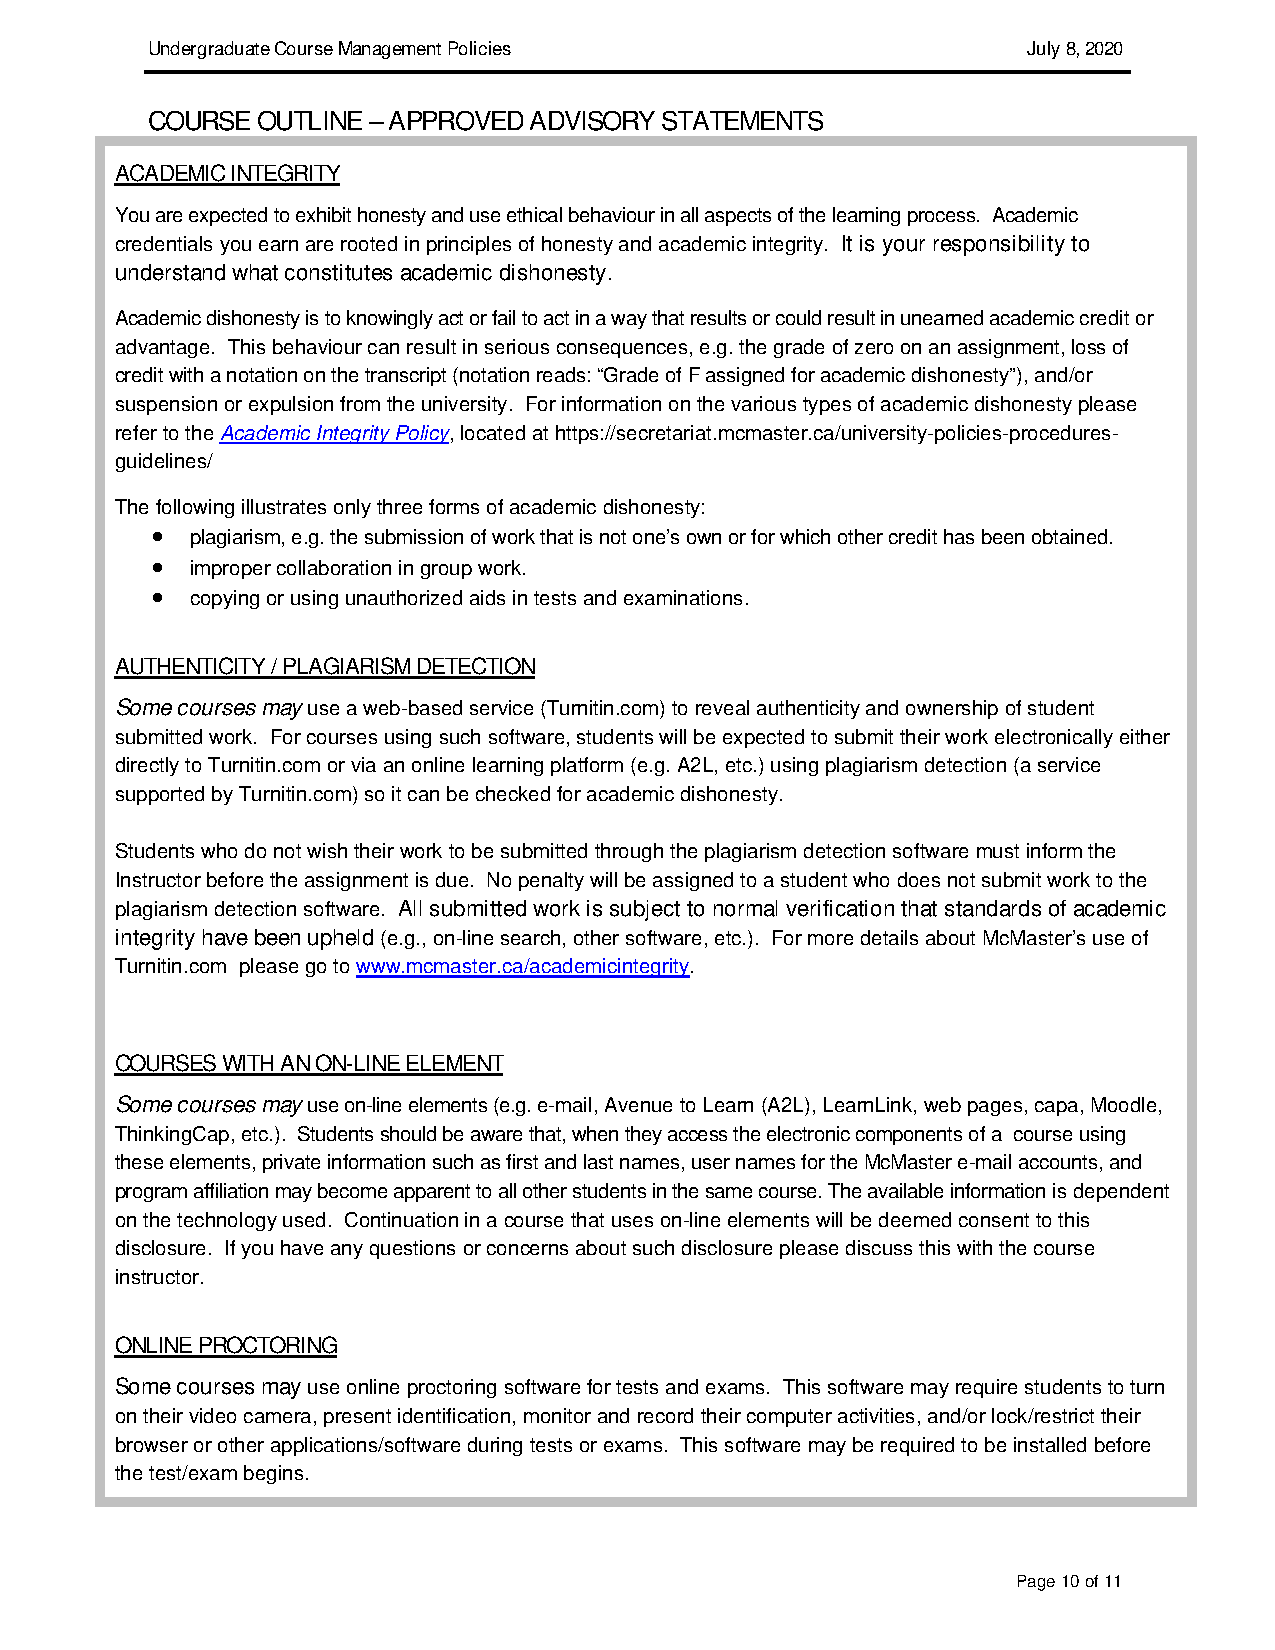
\includepdf[pages=-,width=\pagewidth]{media/outline-advisory-statements.pdf}
\end{document}
